\documentclass[12pt]{report}
\usepackage[a4paper, top=15mm, left=15mm, right=10mm, bottom = 15mm]{geometry}
\usepackage{amsmath, amssymb}
\usepackage{enumerate}
\usepackage{listings, color}
\usepackage{hyperref}
\usepackage{enumerate}
\usepackage{graphics}


\title{CS 202 Review}
\author{Huy Nguyen}
\newcommand{\co}{\texttt}
\renewcommand{\and}{\ \&\& \ }

\lstset{
  backgroundcolor = \color{white},
  frame=tb,
  language=C,
  aboveskip=3mm,
  belowskip=3mm,
  showstringspaces=false,
  columns=flexible,
  basicstyle={\small\ttfamily},
  numbers=none,
  numberstyle=\tiny\color{gray},
  keywordstyle=\color{blue},
  otherkeywords = {},
  commentstyle=\color{red},
  stringstyle=\color{mauve},
  breaklines=true,
  breakatwhitespace=true,
  tabsize=3
}

\begin{document}

\tableofcontents

\chapter[Chapter 3 Solution]{Decomposition of graphs}

\chapter[Chapter 4 Solution]{Distance in graph}

\section{Problem 4.3}
Modify the breadth first search algorithm as follows. Here each node has a property \co{dist}, the length of the shortest path from the source node to it, and a property \co{n}, the number of shortest paths from the source node to it. We update both as we visit each node. If we find a node whose \co{dist = n = 2} then there exists a cycle of length $4$.
\begin{lstlisting}
  bfsModified(Node u):
    For all node v:
      v.dist = INFINITY
      v.n = 0
    u.dist = 0
    H = makeQueue(u)
    while H is not empty:
      Node s = h.poll()
      for all node v adjacent to s:
        if v.dist = INFINITY:
          v.n ++
          v.dist = s.dist + 1
          H.add(v)
        else:
          if s.dist + 1 == v.dist:
            // found another shortest path from u to v
            v.n ++
            if v.n == 2 && v.dist == 2:
              // found a simple cycle of four
              return TRUE
    return FALSE
\end{lstlisting}
We call \co{bfsModified} on all vertices in the graph. The complexity is therefore $O(|V| ( |E| + |V|)) = O(|V|^3)$ because $|E| = O(|V|^2)$.

\section{Problem 4.4}
\begin{center} 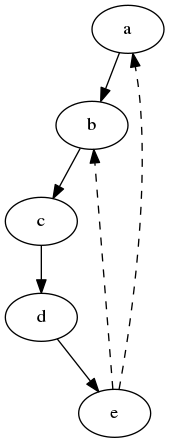
\includegraphics{dfs_fail.png} \end{center}
In the above tree, the cycle edges are $EB$ and $EA$. $EB$ will give \co{level[E] - level[B] + 1 = 4 - 1 + 1 = 4}, while $EA$ will give \co{level[E] - level[A] + 1 = 4 - 0 + 1 = 5}. The shortest cycle, however, is $ABE$ with length $3$. \\
The reason is that dfs can only detect all back edges but not all cycles; a back edge might belong to more than one cycle.

\section{Problem 4.5}
Use the \co{bfsModified} algorithm from 4.3:
\begin{lstlisting}
  bfs_modified(Node u, Node target):
    For all node v:
      v.dist = INFINITY
      v.n = 0
    u.dist = 0
    H = makeQueue(u)
    while H is not empty:
      Node s = h.poll()
      for all node v adjacent to s:
        if v.dist = INFINITY:
          // first time v is discovered, set number of shortest path to 1
          v.n ++
          v.dist = s.dist + 1
          H.add(v)
        else:
          if s.dist + 1 == v.dist:
            // found another shortest path from u to v
            v.n ++
    return target.n
\end{lstlisting}

\section{Problem 4.6}
Consider the directed graph $G'$ formed by taking all the edges $\overrightarrow{(u, \co{prev}[u]}$. We note that the \co{prev} array is set in Dijkstra when
\begin{lstlisting}
  s = H.remove()
  for v adjacent to s:
    if v.dist > s.dist + l(v,s):
      v.dist = s.dist + l(v,s)
      prev[v] = s
\end{lstlisting}
In other words, if we have an edge $\overrightarrow{(a,b)}$ in $G$, then $b = \co{prev}[a]$ so \co{b.dist > a.dist}. So if there is a path from a node $a$ to a node $c$ then \co{c.dist > a.dist}. If there is a cycle then there is an edge from a node $c$ to a node $a$ while there is also a path from $a$ to $c$. The former implies \co{a.dist > c.dist} while the latter implies \co{c.dist > a.dist}, so we have a contradiction.

\section{Problem 4.7}
First get the shortest path distance of all vertices using only the edges in $E'$. Now remove all the edges in $E'$. We are left with the graph $G'(V, E - E')$. Run \co{update} on all edges in $E'$:
\begin{lstlisting}
update(e = (u,v)){
  v.dist = min { v.dist, u.dist + w(e)}
}
\end{lstlisting}
If any vertex has its \co{dist} changed, then the \co{dist} we obtained from $T$ is not correct, so $T$ is not the shortest path tree and we return false. Otherwise, all \co{dist}s are correct so we return true.

\section{Problem 4.8}
Dijkstra's algorithm only cares about the weight of the paths, not their lengths. Adding a constant to the weight of each edge will change the graph, because two paths that previously had same weights but different lengths will not have different weights. \\
Example: Consider $\Delta ABC$ where $AB = -2, BC = 2, CA = 1$. The shortest path from $A$ to $C$ is $A \to B \to C$. If we add $2$ to each edge weight, $AB = 0, BC = 4, CA = 3$ so the shortest path from $A$ to $C$ is now $AC$.

\section{Problem 4.9}
Let $U$ be the set of edges connecting to $S$. Add a large constant to all edges in $U$ so that they all become positive. Since any shortest path from $S$ to any vertex includes exactly one edge in $U$, the relative weight of the shortest paths remain the same, so Dijkstra's algorithm still works.

\section{Problem 4.10}
Run a modified version of Bellman-ford. Because we know no path can have more than $k$ edges, the loop only needs to execute $k$ times, not $|V| - 1$ times. The runtime is therefore $O(k |E|)$.

\section{Problem 4.11}
Use Dijkstra's algorithm to find the shortest cycle going through a given node $n$: After we get the \co{dist} of all nodes from $n$, find $$\min_{u : n \in \co{u.adj}} \{ \co{u.dist} + w(u,s)\}.$$
Call the method on all nodes and find the min of the return values. Dijkstra takes $O(|V|^2)$ and is called $|V|$ times, so the runtime is $O(|V|^3)$.

\section{Problem 4.12}
The length of the shortest cycle containing $e = (u,v)$ is the sum of $w(e)$ and the shortest path from $u$ to $v$. \\
Remove the edge $e = (u,v)$ from the graph and call Dijkstra's on $u$. The result is \co{v.dist} + $w(e)$.

\section{Problem 4.13}
\begin{enumerate}[(a)]
  \item Iterate through $E$ and remove all edges whose lengths are larger than $L$. Then call bfs on $s$ and see if $t$ can be reached.
  \item We use a modified version of Dijkstra's algorithm. Here \co{u.dist} is the maximum edge weight on the path from $s$ to $u$.
  \begin{lstlisting}
    dijkstra(s):
      for all v in V:
        v.prev = null
        v.dist = INFINITY
      s.dist = 0
      H = makeQueue(V)
      while H is not empty:
        u = H.remove()
        for all v adjacent to u:
          if v.dist > max{u.dist, w(u,v)}:
            v.dist = max{u.dist, w(u,v)}
            v.prev = u
  \end{lstlisting}
\end{enumerate}

\section{Problem 4.14}
For all $u, v \in V$ we need to find $d(u,v_0) + d(v_0, v)$. \\
Run Dijkstra's algorithm on $v_0$ we can find $d(v_0, v)$ for all $v \in V$. \\
Consider the reverse graph $G'(V,E')$ such that there is an edge from $u$ to $v$ in $G$ if and only if there is an edge from $v$ to $u$ in $G'$. Run Dijkstra's algorithm on $v_0$ in $G'$ we get $d'(v_0, u)$ for all $u \in V$, which is also $d(u, v_0)$ in the original graph. 

\section{Problem 4.15}
Keep a property \co{count} in each node $u$, which indicates the number of shortest paths from $s$ to $u$. We modify Dijkstra's algorithm as follows:
\begin{lstlisting}
    dijkstra(s):
      for all v in V:
        v.prev = null
        v.dist = INFINITY
        v.count = 0
      s.dist = 0
      s.count = 1
      H = makeQueue(V)
      while H is not empty:
        u = H.remove()
        for all v adjacent to u:
          if v.count == 0:
            // first time v is visited
            v.count ++
          if v.dist > u.dist + w(u,v):
            v.dist = u.dist + w(u,v)
            v.prev = u
          else if v.dist == u.dist + w(u,v):
            // found another shortest path
            v.count ++
\end{lstlisting}
Then, for all $u \in V$, \co{usp[u] = (u.count == 1)}.

\section{Problem 4.17}
\href{http://cs.stackexchange.com/questions/6797/modifying-dijkstras-algorithm-for-edge-weights-drawn-from-range-1-k}{\underline{See link}}

\section{Problem 4.18}
Keep a property \co{count} in each node $u$, which indicates the minimum number of edges in any shortest path from $s$ to $u$. We modify Dijkstra's algorithm as follows:
\begin{lstlisting}
    dijkstra(s):
      for all v in V:
        v.prev = null
        v.dist = INFINITY
      s.dist = 0
      s.count = 0
      H = makeQueue(V)
      while H is not empty:
        u = H.remove()
        for all v adjacent to u:
          if v.dist > u.dist + w(u,v):
            v.dist = u.dist + w(u,v)
            v.prev = u
            v.count = u.count + 1
          else if v.dist == u.dist + w(u,v):
            // found another shortest path
            if v.count > u.count + 1:
              v.count = u.count + 1
              v.prev = u
\end{lstlisting}

\section{Problem 4.19}
Update the weight of all edges as follows:
\begin{itemize}
  \item For all edge $e$ coming from $s: w(e) = w(e) + cost[s]$.
  \item For all edge $e = \overrightarrow{(u,v)}: w(e) = w(e) + cost[v]$.
\end{itemize}
Then disregard the costs of the vertices (because we have moved them to the edges) and run Dijkstra's algorimth on $s$.

\section{Problem 4.20}
The algorithm is as follows:
\begin{itemize}
  \item Run Dijkstra's algorithm on $s$ and $t$. Because the graph is undirected, we get $$d(s,u), d(u,s), d(t,u), d(u,t)$$ for all $t \in V$. Let $d(s,t) = M$.
  \item For each edge $e = (u,v) \in E'$, calculate the length of the shortest path from $s$ to $t$ that includes $e$. This number is $$f(e) = \min \{ d(s,u) + w(e) + d(v,t), d(s,v) + w(e) + d(u,t) \}.$$
  \item Compare $f(e)$ to $M$ and update $M = \min \{ M, f(e) \}$.
\end{itemize}

\section{Problem 5.21}
\begin{enumerate}[(a)]
\item Create a currency trading graph $G(V,E)$:
\begin{itemize}
  \item For each currency $i$ there is a node $v_i \in V$.
  \item For all $u, v \in V (u \ne v)$ there is an edge from $u$ to $v$.
  \item For all $v_i, v_j \in V: w(v_i, v_j) = \log \frac{1}{r_{i,j}} = - \log r_{i,j}$.
\end{itemize}
Therefore if $d = w(i,j)$ then one unit of $c_i$ can be converted into $2^d$ units of $c_j$.
The best way to convert from $s$ to $t$ is the shortest path from node $v_s$ to $v_t$ in $G$, which can be found by Bellman-Ford's algorithm.

\item
The existence of an anomaly implies that $$r_{i_1, i_2} \cdot r_{i_2, i_3} \cdot \ldots \cdot r_{i_k, i_1} > 1,$$
which is equivalent to $$\log \frac{1}{r_{i_1, i_2}} +  \log \frac{1}{r_{i_2, i_3}} +  \ldots + \log \frac{1}{r_{i_k, i_1}} < 0.$$
In other words, $$w(v_{i_1}, v_{i_2}) + + w(v_{i_2, v_{i_3}}) + \ldots + w(v_{i_k}, v_{i_1}) < 0,$$
So we have a negative cycle $i_1 \to i_2 \to i_3 \to \ldots \to i_k \to i_1.$ \\
To detect if a negative cycle exists, use Bellman-Ford's algorithm. If it returns YES, there is an anomaly. Otherwise, there isn't.
\end{enumerate}
\chapter[Chapter 5 Solution]{Greedy algorithm}

\section{Problem 5.3}
Run DFS on the graph to detect a cycle edge. Return YES as soon as a cycle edge is found. Else, if there is no cycle edge, return NO.\\
This algorithm has $O(|V|)$ runtime because we note that $G$ is either a tree (in which case $|E| = |V| - 1$) or it is not (in which case $|E| > |V| - 1)$.
\begin{itemize}
  \item If $G$ is a tree then we will not be able to detect any back edge. DFS will traverse the entire graph, which takes $O(|V| + |E|)$, but because $|E| = |V| - 1$, this is $O(|V|)$.
  \item If $G$ is not a tree then we can find a back edge after traversing at most $|V|$ edges because the edges picked by DFS form a tree, and any tree in the original graph can have at most $|V|$ vertices.
\end{itemize}

\section{Problem 5.4}
We note that a connected component with $m$ vertices must have at least $m - 1$ edges\footnote{since the component is connected, we can build a minimum spanning tree in it; this tree has $m$ vertices and $m-1$ edges, so the number of edges in the component must be at least $m-1$.}. \\
Let the number of vertices in component $i$ be $m_i, \ i = 1,2,\ldots,k$. We have $\displaystyle \sum_{i=1}^k m_i = n$.\\
The number of edges in the graph is the total number of edges in all components, which is at least $$\sum_{i=1}^k (m_i - 1) = n - k.$$


\section{Problem 5.5}
\begin{enumerate}[(a)]
  \item We follow Kruskal's algorithm to build the minimum spanning tree: at each step, pick the edge with the least weight that does not create a cycle. Because all edge weights are increased by $1$, the weight of any edge relative to all other edges is the same, so Kruskal's will produce the same result.
  \item The shortest path will change. Consider the quadrilateral $ABCD$ with $$AB = BC = CD = 2, AD = 7.$$ Currently the shortest path from $A$ to $D$ is $A \to B \to C \to D$. If we increase the weight of all edges by $1$ then $AB = BC = CD = 3, DA = 8$, so the shortest path from $A$ to $D$ is $A \to D$.
\end{enumerate}

\section{Problem 5.6}
Sort the edge by their weights $$e_1 < e_2 < \ldots < e_n.$$
Kruskal's algorithm will iterate $n$ times and, at time $i$, pick edge $e_i$, or the $i-$th smallest edge in the graph. Because the edge weights are distinct, the $i-th$ smallest edge in the graph is distinct for all $1 \le i \le n$. Therefore the minimum spanning tree is unique.

\section{Problem 5.7}
Negate all the edge weights in the input graph and use Kruskal's algorithm to find the minimum spanning tree in the new graph. This tree is the maximum spanning tree in the original graph.

\section{Problem 5.8}
We use Prim's algorithm to build a minimum spanning tree in $G$. \\
Start building the MST from a vertex that is not $S$. Now assume we have reached the step where we have the tree current tree $T$ and we are about to add $S$ to $T(V)$. In other words, the next edge to be added to $T(E)$ is the edge $SA$ connecting $S$ to a vertex $A \in T(V)$, which means $SA$ is the lightest edge that connects $T$ a vertex outside of $T$. $(*)$\\
We prove that $SA$ is also the shortest path from $S$ to $A$ and therefore $T$ and the tree of shortest paths from $S$ share the same edge $SA$. \\
Assume otherwise, the shortest path from $S$ to $A$ is not $SA$. Then there exists a vertex $B \ne A$ such that the shortest path from $S$ to $A$ consists of the shortest path from $S$ to $B$ and $BA$. So $$d(S,B) + BA < SA.$$
We consider two cases:
\begin{itemize}
  \item If $B \notin T(V)$ then because $BA < SA$, $SA$ is not the lightest edge that connects $T$ to a vertex outside of it.
  \item If $B \in T(V)$, call $I$ and $K$ two vertices on the path from $S$ to $B$ such that $I \in T(V), K \notin T(V)$ ($I$ can be $B$ and $K$ can be $S$). Then $SA > d(S,B) = d(S,K) + IK + d(I,B) \ge IK$, so again $SA$ is not the lightest edge.
\end{itemize}
Both cases contradict $(*)$. Thus we have proven that the minimum spanning tree and the tree of shortest paths from a vertex $S$ always share an edge.

\section{Problem 5.10}
Start with a MST $T_H \in MST_H$ and $T_G \in MST_G$. \\
While there is an edge $e \in T_G \bigcap H$ such that $e \notin T_H$ do:
\begin{enumerate}
  \item Add $e$ to $T_H$ to create a cycle $C$.
  \item We see that for all $e' \in C, e' \ne e$ we have $w(e') \le w(e)$. Otherwise if $w(e') > w(e)$ we should have picked $e$, not $e'$ when building the MST $T_H$, according to Kruskal's algorithm.
  \item Let $e = (u,v)$, so $u, v \in H$. We see that $e \in T_G$ so it connects two previously separate connected components, which we call $U$ and $V$, and assume that $u \in U, v \in V$. Because $u$ and $v$ are in $H$ and $T_H$ is the MST of $H$, there exists an edge $e'' \in C \bigcap T_H$ that connects $U$ and $V$. 
  \item From Step 2 we get $w(e'') \le w(e)$. If $w(e'') < w(e)$ then when we built $T_G$ we should have picked $e''$ instead of $e$ to connect $U$ and $V$. Therefore $w(e'') = w(e)$. 
  \item Let $T'_H = T_H \bigcup \{ e \} - \{ e''\}$ then $T_H$ is also a MST in $H$.
  \item Rename $T'_H \to T_H$ and check the loop condition.
\end{enumerate}

After the loop we have $T_G \bigcap H \subset T_H$.

\section{Problem 5.16}
\href{http://ocw.mit.edu/courses/electrical-engineering-and-computer-science/6-046j-design-and-analysis-of-algorithms-spring-2012/assignments/MIT6_046JS12_ps9_sol.pdf}{\underline{See link}}

\section{Problem 5.20}
{\bf Perfect matching.} \\
Let $G(V,E)$ be the input graph, $S$ be the queue that contains all leaf nodes and $M$ be the perfect matching. \\
The algorithm is as follows:
\begin{lstlisting}
  all leaf nodes to S.
  while S is not empty:
    u = S.pop()
    v = u.adjacent
    M.add((u,v))
    Remove u, v from V and all edges connected to v from E
    Add new leaf nodes to S
  return |V| = 0
\end{lstlisting}
{\bf Feedback edge set.} \\
Let $F$ be the feedback edge set. Negate all the edges in $G$ to get a graph $G'$. Use Kruskal's algorithm to build a minimum spanning tree $T$ in $G'$. At each step, after we pop an edge $e$, if adding $e$ to $T$ does not form a cycle, then add $e$ to $T$, else add $e$ to $F$. As we go back to the original graph, $T$ is the maximum spanning tree and $F$ is the feedback set edge with minimum weight.

\section{Problem 5.21}
\begin{enumerate}[(a)]
\item If no MST contain $e$, we are done. If {\bf there is a MST $T$ that contains $e$}, removing $e$ from $T$ will separate it into two connected components $M$ and $N$. Since $e$ is part of a cycle, there exists another edge $e'$ that connects $M$ and $N$. Then $T \bigcup \{ e' \} - \{e\}$ is also a MST with $w(T') \le w(T)$. 
\begin{itemize}
  \item If $w(T') < w(T)$ then we have a contradiction because $T$ is a MST, so no MST can contain $e$. 
  \item If $w(T') = w(T)$ then $e$ and $e'$ are both the heaviest edges in the cycle. $T$ contains $e$ and not $e'$, while $T'$ contains $e'$ and not $e$. In other words, there is a MST that does not contain the heaviest edge in a cycle.
\end{itemize}
\item If we get an edge $e$ that is part of a cycle, then because the edges are ordered in decreasing weights, $e$ is the heaviest edge in that cycle. By the property in (a), $e$ cannot belong a MST. Therefore we can remove it.
\item To check if an edge $e$ belongs to a cycle:
  \begin{itemize}
    \item Let $e = (u,v)$.
    \item Remove $e$ from the graph and DFS on $u$.
    \item If $v$ can be reached, return YES. Else, return NO.
  \end{itemize}
\item The loop executes $E - (|V| - 1)$ times because that is the number of edges we need to remove to get a MST with $|V|$ vertices and $|V| - 1$ edges. Each iteration takes $O(|V| + |E|)$ times because of DFS. Therefore the total runtime is $$O( (|V| + |E|) \cdot (|E| - |V| + 1)).$$
\end{enumerate}


\section{Problem 5.23}
The algorithm can be described as follows:
\begin{itemize}
  \item Let $E'$ be the set of all edges that touch a vertex in $U$.
  \item Build a MST $T$ in $G'(V - U, E - E')$.
  \item For each node $u$ in $U$, add the lightest edge that connects $u$ and $T$ to $T$.
  \item Return $T$.
\end{itemize}

\section{Problem 5.29}
\href{www.ece.northwestern.edu/~dda902/336/hw5-sol.pdf}{\underline{See link}}

\chapter[Chapter 6 Solution]{Dynamic programming}
\section{Problem 6.2}
Let $b[i]$ be the minimum total penalty for stopping at hotel $a_i$, $1 \le i \le n$. We have $$b[i] = \min_{1 \le j < i} \{ b[j] + (200 - (a[i] - a[j]))^2\}.$$
Also record the value $j$ which yields $\displaystyle \min_{1 \le j < i} \{ b[j] + (200 - (a[i] - a[j]))^2\}$ and set \co{b[i].prev = b[j]}. Backtrack from $b[n]$ to get the sequence of hotels to stop by.


\section{Problem 6.3}
Let $S[i]$ be the maximum total profit we get from building some restaurants in $\{m_1, m_2, \ldots, m_i\}$. Consider 2 cases:
\begin{enumerate}[(1)]
  \item If restaurant $m_i$ should not be built, then $S[i] = S[i-1]$.
  \item If restaurant $m_i$ should be built, then let $c_i$ be the maximum index $j$ which yields $m_i - m_j \ge k$. We then have $\displaystyle S[i] = p_i + S[c_i]$.
\end{enumerate}
Therefore in general, $$S[i] = \max \{ S[i-1], p_i + S[c_i]\}.$$
To get the sequence of restaurants, keep an array $R[n]$ such that $R[i] = 1$ if restaurant $i$ is built in the optimal solution, and $R[i] = 0$ otherwise. When we calculate $S[i]$, if the max falls to case (1), $R[i] = 0$. Else, $R[i] = 1$. Output all the $R[i]$s that are $1$.

\section{Problem 6.4}
Consider an array $S[n]$ where $S[i] = \co{true}$ if the substring $s_1 s_2 \ldots s_i$ is a valid string, and \co{false} otherwise. We have $S[1] = \co{dict(s[1])}$ and 
$$
\begin{aligned}
S[i] = & \ (S[1] \and \co{dict(s[2 .. i]}) \\ 
& || (S[2] \and \co{dict(s[3..i])} \\ 
& || \ldots \\
& || (S[i-1] \and \co{dict(s[i..i])})), 
\end{aligned}$$
where $s[j..i]$ is $s_j s_{j+1} \ldots s_i$.


\section{Problem 6.5}
\begin{enumerate}[(a)]
\item Consider a column of $4$ squares. There can be either $0$ pebble, or $1$ pebble (4 ways to place it), or $2$ pebbles (either place it on square $1$ and $3$ or $2$ and $4$). Therefore there are a total of $7$ patterns on a column.
\item Let $T[i,j]$ be the max sum we get from putting pebbles on the table from from column $1$ to $i$ using the pattern $j$. Let $C(i,j)$ be the value we get when putting a pebble on square $(i,j)$. We have $$T[i,j] = C(i,j) + \max \{ T[i-1,j'] \}, $$
where $j' \in \{0,1,\ldots,6\}$ and pattern $j'$ is compatible with pattern $j$.
\end{enumerate}

\section{Problem 6.6}
Let the input string be $x_1 x_2 \ldots x_n$. \\
Let $Z = \{a,b,c\}$ and let $T[i,j] \subset Z$ be the set of the possible values that the product $x_i x_{i+1} \ldots x_{j}$ can yield with all possible parenthesizations. \\
We see that $T[i,i] = x_i$ for all $1 \le i \le n$. We need to compute $T[1,n]$. \\
Define $A \times B$ as $\{ a \cdot b | a \in A, b \in B\}$. \\
We note that $$T[i, i+1] = T[i,i] \times T[i+1, i+1]$$ and $$T[i,i+2] = (T[i,i] \times T[i+1, i+2]) \bigcup (T[i,i+1] \times T[i+2,i+2]).$$
(to put it another way, $xyz$ can be written as $(x)(yz)$ or $(xy)(z)$) \\
We therefore see that we already have $$T[1,1], T[2,2], T[3,3], \ldots,$$
from which we can calculate $$T[1,2], T[2,3], T[3,4], \ldots,$$
from which we can calculate $$T[1,3], T[2,4], T[3,5], \ldots $$
and eventually we can expand to $T[1,n]$, which is what we need to find.\\
In other words, $$T[i, i + s] = \bigcup_{i \le k < i + s} (T[i,k] \times T[k+1, i + s]).$$
The algorithm is as follows:
\begin{lstlisting}
  for i = 1 to n: 
    T[i,i] = x[i].
  for s = 1 to n-1:
    for i = 1 to n - s:
      T[i, i + s] = empty
      for k = 1 to i + s - 1:
        T[i, i + s] = T[i, i + s] UNION (T[i, k] * T[k+1,s])
  If a is in T[1,n] return true. Else, return false.
\end{lstlisting}

\section{Problem 6.7}
Let the input string be $x_1 x_2 \ldots x_n$. Let $T[i,j]$ be the length of the longest palindromic subsequence in $x[i..j]$. We have $$\begin{cases} T[i.i] = 1 \\ T[i,i+1] = 2 \text{ if } x[i] = x[i+1] \text{ and } 0 \text{ if } x[i] \ne x[i+1] \\ T[i,j] = T[i+1,j-1] + 2 \text{ if } x[i] = x[j] \text{ and } \max \{T[i+1,j], T[i,j-1]\} \text{ else} \end{cases}$$

\section{Problem 6.8}
Let $E[i,j]$ be the length of the largest common substring of $x_1 x_2 \ldots x_i$ and $y_1 y_2 \ldots y_j$ such that $x_i = y_j$. We see that $E[1,j] = 1$ if $x_1 = y_j$ and $0$ otherwise. Similarly, $E[j,1] = 1$ if $y_1 = x_j$ and $0$ otherwise.\\
In general, we have $$E[i,j] = \begin{cases} E[i-1,j-1] + 1 \text{ if } x_i = y_j \\ 0 \text{ if } x_i \ne y_j \end{cases}$$

\section{Problem 6.9}
Let the input string be $x[0..n-1]$ and the input breakpoint array be $y[1..m]$. Convert $y$ to $y[0..m+1]$ and let $y[0] = -1, y[m+1] = n-1$. \\
Let $M(i,j)$ be 
$$\begin{cases} M(i,i)=0\text{, }\forall i: 0 \le i \le m + 1 \\
M(i,i + 1)=0\text{, }\forall i: 0 \le i \le m + 1\\
M(i,j)=\left(y[j]-y[i]\right) + \displaystyle \min_{l: i < l < j}\{M(i,l) + M(l,j)\}
\end{cases}$$

\section{Problem 6.10}
Let $E[i,j]$ be the probability of obtaining exactly $i$ heads when $j$ coins $c_1, c_2, \ldots, c_j$ with head-probability $p_1, p_2, \ldots, p_j$ are tossed.
We have $$\begin{cases} E[0,0] = 1 \\ E[0,j] = E[0,j-1] \cdot (1-p_j) \ \forall 1 \le j \le n \\ E[i,0] = 0 \ \forall 1 \le i \le k \\ E[i,j] = p_j \cdot E[i-1,j-1] + (1-p_j) \cdot E[i,j-1] \end{cases}$$

\section{Problem 6.11}
Let $E[i,j]$ be the longest common subsequence of $x_1 x_2 \ldots x_j$ and $y_1 y_2 \ldots y_j$. \\
We have $E[1,j] = 1$ if $x_1 = y_j$, for all $1 \le j \le m$. Similarly, $E[j,1] = 1$ if $x_j = y_1$, for all $1 \le j \le n$. \\
In general we have $$E[i,j] = \begin{cases} E[i-1,j-1] + 1 \text{ if } x_i = y_j \\ \max \{E[i-1,j] + E[i,j-1] \} \text{ if } x_i \ne y_j. \end{cases}$$

\section{Problem 6.12}
Let $d[i,j]$ be the distance between point $i$ and $j$. We have $$\begin{cases} A[i,i] = 0 \\ A[i, i + 1] = 0 \\ A[i, i+2] = 0 \\ A[i,j] = \displaystyle \min_{i < k < j} \{ A[i,k] + A[k,j] + d[i,k] + d[k,j]\} \end{cases}$$

\section{Problem 6.13}
A sequence where a greedy approach would fail is $$1000 \quad 2000 \quad 500 \quad 1.$$
Let $E[i,j]$ be the maximum value the first player can have by picking cards from the set of cards $s_i, s_{i+1}, \ldots, s_j$. \\
We see that $E[i,j] = 0$ if $i \le j$. In general, $$\begin{aligned} E[i,j] = \max\{ & v_i + \min \{ E[i + 2, j] - v_{i+1}, E[i + 1, j - 1] - v_j \}, \\ & v_j + \min \{ E[i+1,j-2] - v_{j-1}, E[i+2,j-1] - v_{i+1}\}\}. \end{aligned}$$
\end{document}